\documentclass[a4paper, 11pt]{article}
\usepackage[T1]{fontenc}
\usepackage[portuguese]{babel}
\usepackage[utf8]{inputenc}
\usepackage[margin=2cm,includefoot,includehead,footskip=30pt]{geometry}

\usepackage{graphicx}
\graphicspath{ {imagens/} }
\usepackage{bold-extra}
\usepackage{epstopdf}
\usepackage{float}
\usepackage{scalerel}
\usepackage{enumerate}
\usepackage{indentfirst}
\usepackage{cleveref}
\usepackage{amssymb}
\usepackage{listings}
\usepackage{color}
\usepackage{imakeidx}
\newcommand\showdiv[1]{\overline{\smash{\hstretch{.5}{)}\mkern-3.2mu\hstretch{.5}{)}}#1}}
\newcommand\ph[1]{\textcolor{white}{#1}}


\lstset{frame=tb,
  language=Matlab,
  aboveskip=3mm,
  belowskip=3mm,
  showstringspaces=false,
  columns=flexible,
  basicstyle={\small\ttfamily},
  numbers=none,
  numberstyle=\tiny\color{gray},
  keywordstyle=\color{blue},
  commentstyle=\color{dkgreen},
  stringstyle=\color{mauve},
  breaklines=true,
  breakatwhitespace=true,
  tabsize=3,
  extendedchars=true,
  literate=	{á}{{\'a}}1	{ã}{{\~a}}1	{â}{\^{a}}1	{é}{\'{e}}1	{ç}{\c{c}}1
  			{ã}{\~{a}}1	{à}{\`{a}}1 {ê}{\^{e}}1 {í}{\'{i}}1	{ó}{\'{o}}1
  			{õ}{\~{o}}1 {ô}{\^{o}}1	{ú}{\'{u}}1 {Ç}{\c{C}}1,
}

\addto\captionsportuguese{
  \renewcommand{\contentsname}%
    {Índice}%
}

% ----- Cabeçalho e rodapé -----
\usepackage{fancyhdr}
\pagestyle{fancy}
\fancyhf{}

\renewcommand{\headrulewidth}{0.5pt}
\renewcommand{\footrulewidth}{0.5pt}

\rhead{Wordmorph}
\lhead{Algoritmos e Estruturas de Dados\rightmark}
\rfoot{Página \thepage}
\lfoot{\small Engenharia Electrotécnica e de Computadores - IST}


\usepackage{pdfpages}

\begin{document}


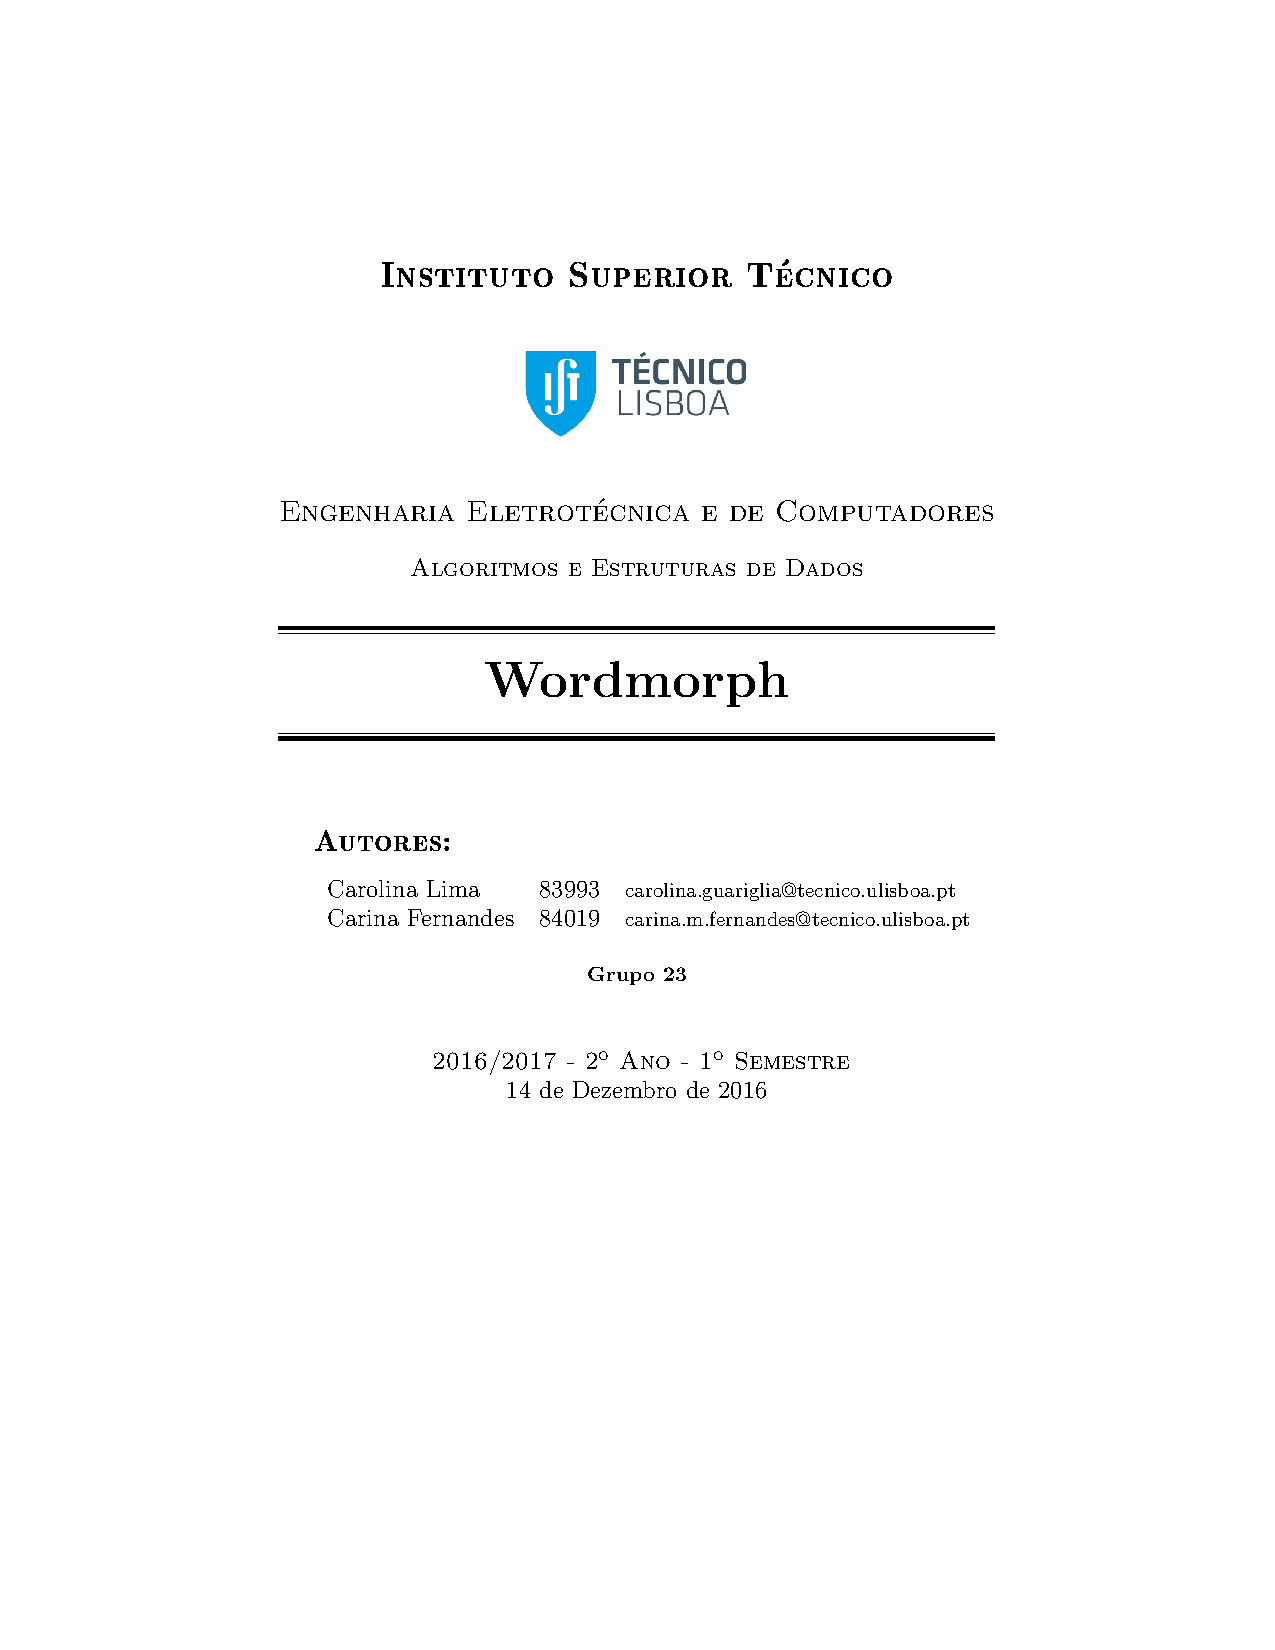
\includepdf[pages={1}]{capa/capa.pdf}

\tableofcontents{}
\newpage

\section{Descrição do problema}
    \par O problema enunciado consiste na procura de caminhos entre palavras. Estes caminhos são, na verdade, uma sequência de palavras de tamanho igual no qual cada palavra se obtêm mudando uma ou mais letras da palavra anterior, até chegar à palavra desejada. Para além disso, todas as palavras pertencentes ao caminho têm obrigatoriamente de pertencer a um dicionário. Dicionário é definido neste caso como uma lista de palavras, que não têm obrigatoriamente de ser todas do mesmo tamanho.
    \par Como é possível a existência de vários caminhos, distingue-se cada passo do caminho pelo número de caracteres que são mudados. No fim, os custos dos caminhos somam-se para chegar ao custo final. Por exemplo, um passo no qual se mude um caracter têm o custo de $1^1$, um passo em que se mudam dois caracteres têm um custo de $2^2$, e assim sucessivamente.
    \par O objectivo final deste projecto é, dado duas palavras e o número máximo de trocas que se podem efectuar em cada passo, retornar o caminho de menor custo entre essas duas palavras.
    
\section{Abordagem do problema}
    \par Para resolver o problema, decidiu-se dividi-lo nas seguintes partes: guardar as palavras do dicionário e procurar o caminho propriamente dito. Logo chegou-se à conclusão de que seria necessário guardar as palavras do dicionário num local que fosse facilmente acessível. 
\subsection{Procura do caminho de menor custo}
    \par A escolha óbvia para resolver este problema foi recorrer ao algorítmo de Dijkstra, que procura o caminho mais curto entre dois vértices de um dado grafo desde que nenhuma das arestas do mesmo tenha peso negativo, o que é o caso deste problema. Para podermos utilizar então o algorítmo, foi necessária a criação de um grafo representado por listas de adjacências (o algorítmo não é igual para matrizes de adjacência).
    \par Note-se também que cada conjunto de palavras de um dado tamanho vai requerer o seu próprio grafo.
    
\section{Implementação do programa}
    \par Dividiu-se então o programa em três partes distintas: uma parte referente às estruturas de dados, uma parte que se relaciona diretamente com o problema a resolver, e por fim todas as restantes operações que não pertencem a nenhum dos anteriores grupos. No código, estas partes equivalem aos ficheiros datastructs.c, words.c e utils.c respectivamente.
    
\subsection{Descrição das estruturas de dados}
    \par Como referido acima, era claro que seria necessária a criação de uma lista de adjacências, então foi implementada uma lista genérica. Esta é definida usando void * (definido em datastructs.h como sendo Item), para os quais se pode passar qualquer ponteiro, assegurando a generalidade da implementação.
    \par As listas definidas foram então utilizadas na definição do grafo pois este é implementado usando uma lista de adjacências. Os grafos foram definidos de forma genérica, com um reparo - a implementação dos dados usados na lista estão visíveis ao cliente.  
    \par Por fim, a descrição do algorítmo de Dijkstra requer um acervo, que neste caso foi implementado usando uma fila prioritária, também esta definida de forma genérica no código.

\section{Complexidade do programa}

\section{Exemplo}


\end{document}
